\documentclass[10pt,twocolumn,letterpaper]{article}
\usepackage[pagenumbers]{cvpr}

\usepackage{graphicx}
\usepackage{booktabs}
\usepackage{amsmath}
\usepackage{amssymb}
\usepackage{multirow}
\usepackage{xcolor}
\definecolor{cvprblue}{rgb}{0.21,0.49,0.74}
\usepackage[pagebackref,breaklinks,colorlinks,allcolors=cvprblue]{hyperref}
\newcommand{\todo}[1]{\textcolor{red}{[TODO: #1]}}

\title{Multi-View 3D Reconstruction from Sparse to Dense Views:\\
COLMAP versus VGGT and Depth Anything 3 on ETH3D}

\author{Shunyang Huang\qquad Mingyu Lin}

\begin{document}
\maketitle

\begin{abstract}
We compare a classical multi-view reconstruction pipeline, COLMAP, with two recent feed-forward models,
VGGT and Depth Anything 3 (DA3), on the 11 scenes of the ETH3D high-resolution benchmark. We vary the number of
input views from 5 to all images of a scene and their overlap, and evaluate camera poses, the accuracy and
completeness of the dense geometry, runtime and GPU memory with the same images and the same evaluation for
every method. DA3 gives the best geometry in every setting. COLMAP produces the most accurate points, but it
reconstructs less than half of the visible surface and often fails when the views overlap little: with five
random views it registers fewer than half of the images. On the images it does register, its cameras are the most
accurate, and with all views it gives the best poses overall. More input views improve COLMAP's cameras, while
the feed-forward models do not gain from additional views on a fixed set of images. The feed-forward models are
20 to 240 times faster but need up to 3.5 times more GPU memory. An attempt to combine both families did not
improve on DA3.
\end{abstract}

%-------------------------------------------------------------------------
\section{Introduction}

Multi-view 3D reconstruction estimates the camera poses of a set of images and the geometry of the scene
they show. For two decades the standard solution has been a pipeline of classical image processing and
geometry: local features are detected and matched across images, the cameras are estimated by
structure-from-motion (SfM) with bundle adjustment, and dense depth is computed by multi-view stereo (MVS).
COLMAP~\cite{schonberger2016sfm,schonberger2016mvs} is the most widely used implementation of this pipeline.

Recently, large transformers trained on many 3D datasets have started to solve the same task in a single
forward pass. VGGT~\cite{wang2025vggt} and Depth Anything 3 (DA3)~\cite{lin2025da3} take a set of unposed
images and directly predict the camera of every image and a dense depth map for it. They run in about a
second and never fail to return a result, but they work on images of about 500 pixels width and do not
optimize the geometry explicitly.

The two families have different strengths and failure modes, and it is not obvious which one to use when
only a few images are available. In this project we compare them on the same data, the ETH3D high-resolution
multi-view benchmark~\cite{schops2017eth3d}, and vary two factors that matter in practice: the number of
input views (5, 10, 20 and all images of a scene) and their overlap (spatially neighboring views versus random
views). We measure the
quality of the recovered cameras, the accuracy and the completeness of the geometry, and the runtime.

DA3 gives the best geometry in every setting and VGGT the second best. COLMAP's points are the most
accurate, but it covers much less of the surface, and with low-overlap views it often cannot register the images
at all. Its cameras, in contrast, are the most accurate on the images it registers and the best overall when all
views are used. More views make COLMAP's cameras better; on a fixed set of views, the feed-forward models do not
gain from more input views, and VGGT's cameras become worse. The learned models need seconds instead of minutes,
at the cost of more GPU memory.

%-------------------------------------------------------------------------
\section{Related Work}

\paragraph{Classical SfM and MVS.}
Incremental SfM registers images one by one: it starts from a well-conditioned image pair, adds images by
solving perspective-n-point problems against already triangulated points, triangulates new points and refines
everything by bundle adjustment~\cite{schonberger2016sfm}. Dense MVS then estimates a depth map per image.
PatchMatch-based methods~\cite{schonberger2016mvs} propagate depth and normal hypotheses between neighboring
pixels and select, per pixel, the source images that see the same surface.

\paragraph{Feed-forward 3D reconstruction.}
DUSt3R~\cite{wang2024dust3r} showed that a transformer can regress a point map for a pair of images without
known cameras; multi-view reconstruction then still needs a global alignment step. VGGT~\cite{wang2025vggt}
processes all images jointly with alternating frame-wise and global attention and predicts cameras, depth maps
and point maps for all of them in one pass. DA3~\cite{lin2025da3} uses a plain vision transformer and a
depth-and-ray representation and reports large gains over VGGT on pose and geometry benchmarks, including
ETH3D.

%-------------------------------------------------------------------------
\section{Methods}

\subsection{Traditional method: COLMAP}
\label{sec:colmap}

We run the standard COLMAP pipeline with its default parameters.

\paragraph{Feature extraction.}
SIFT~\cite{lowe2004sift} builds a Gaussian scale space for each image and detects keypoints as extrema of the
difference of Gaussians across position and scale. Each keypoint receives a dominant orientation from the
local gradient histogram and a 128-dimensional descriptor of gradient orientations in a $4\times4$ grid around
it, which makes it invariant to scale and rotation and robust to illumination changes. Images are processed at
up to 3200 pixels on the longer side.

\paragraph{Matching and geometric verification.}
All image pairs are matched by nearest-neighbor search on the descriptors with Lowe's ratio test and mutual
consistency. For each pair, RANSAC~\cite{fischler1981ransac} estimates the fundamental, essential and
homography matrices; only matches consistent with the epipolar geometry are kept.

\paragraph{Incremental SfM.}
Starting from a pair with many verified matches and a wide baseline, images are registered one at a time by
solving the perspective-n-point problem with RANSAC, new points are triangulated, and the reconstruction is
refined by bundle adjustment, \ie by minimizing the reprojection error over all cameras, intrinsics and 3D
points with a robust loss. An image that cannot be registered is left out of the reconstruction.

\paragraph{Dense reconstruction.}
The registered images are undistorted and resized to 1600 pixels on the longer side. PatchMatch
stereo~\cite{schonberger2016mvs} estimates a depth and a normal per pixel by propagating hypotheses across the
image and scoring them by the normalized cross-correlation of image patches warped into up to 20 source images;
a second pass enforces geometric consistency between the depth maps of different images. Finally, stereo fusion
merges the depth maps into a point cloud, keeping a point only if enough images agree on it within 1\% depth and
$10^\circ$ normal tolerance.

\subsection{Advanced methods: VGGT and DA3}

\paragraph{VGGT.}
VGGT~\cite{wang2025vggt} (1.2B parameters) patchifies each image with a DINO encoder and processes the tokens
of all images with 24 layers that alternate between attention within each frame and attention across all
frames. A camera head predicts the intrinsics and extrinsics of every image, and a DPT head predicts a depth map.
Images are resized to 518 pixels width.

\paragraph{DA3.}
DA3~\cite{lin2025da3} uses a plain DINOv2 transformer with cross-view attention in its later layers and predicts
a depth map and a ray map per image, from which the cameras are recovered. We use the
DA3-Nested-Giant-Large model, which adds a monocular metric depth branch, at the default 504 pixel
resolution.

For both models we use the released weights without fine-tuning. All methods run on one NVIDIA A100 (40\,GB)
GPU.

%-------------------------------------------------------------------------
\section{Experimental Setup}

\subsection{Data and view sampling}

ETH3D~\cite{schops2017eth3d} provides DSLR images of $6048\times4032$ pixels of indoor and outdoor scenes,
with camera poses and depth maps rendered from laser scans. We use the 11 scenes of the DA3
benchmark~\cite{lin2025da3} (14 to 76 images per scene). Neither VGGT nor DA3 was trained on ETH3D.

For each scene we draw subsets of 5, 10 and 20 images with two schemes: \emph{neighbor} subsets consist of a
random anchor image and the images closest to it in camera position and viewing direction, so that the views
overlap strongly; \emph{random} subsets are drawn uniformly, so overlap is left to chance and is often low.
Ground-truth poses are used only to select the subsets. Each setting is repeated with three random seeds.
Three scenes have 20 or fewer images and are not used for 20-view subsets, which gives 180 subsets. In addition,
every scene is reconstructed from all of its images (34 on average). All methods receive exactly the same
images.

\subsection{Evaluation}

\paragraph{Cameras.}
For every pair of input images we compute the angle between the predicted and the ground-truth relative
rotation and between the relative translation directions, and report the area under the curve of the larger
of the two errors up to $5^\circ$ and $30^\circ$ (AUC@5, AUC@30). These relative errors need no alignment.
Pairs involving an image that COLMAP failed to register count as failures.

\paragraph{Geometry.}
Each method is evaluated on its standard dense output: the stereo-fusion point cloud for COLMAP, and the
back-projected depth maps for VGGT and DA3, resampled to the same 1600-pixel grid as COLMAP's depth maps.
Only pixels with ground-truth depth are used. The reconstruction is aligned to the ground truth by a similarity
transform estimated from per-pixel correspondences between predicted and ground-truth 3D points, and refined by
similarity ICP as in the Tanks and Temples benchmark~\cite{knapitsch2017tanks}. Both steps use the
Umeyama solution~\cite{umeyama1991} with iterative outlier trimming. After 5\,mm voxel downsampling, accuracy is
the distance from each predicted point to the ground-truth point cloud, and completeness the distance from each
ground-truth point visible in the input images to the prediction. We report precision, recall and F-score at
2, 5 and 10\,cm. A reconstruction with fewer than three registered images counts as failed (F-score 0).

\paragraph{Ground truth.}
The ground-truth point cloud is the union of the back-projected ground-truth depth maps of all images of the
scene. Its internal consistency sets a floor on the meaningful thresholds: the median distance between one
view's points and those of the other views is 2\,mm indoors and 7--8\,mm outdoors, so 2\,cm is close to the
ground-truth noise outdoors and 5\,cm is our main threshold.

\paragraph{Sanity check.}
To verify our implementation we also run the evaluation protocol of the DA3 benchmark (all views, alignment on
camera centers, TSDF fusion, F-score at 25\,cm) and compare with the published numbers.

\paragraph{Differences to the DA3 protocol.}
We did not use the DA3 protocol for the main comparison for three reasons, each checked on our data.
(i) Its ground-truth mesh misses much of the scanned surface (on one \emph{courtyard} image only 6\% of the rays
through pixels with ground-truth depth hit the mesh). (ii) TSDF fusion extracts little surface from COLMAP's
sparse, consistency-filtered depth maps, which strongly understates COLMAP's completeness. (iii) Aligning on
camera centers is ill-conditioned when the input cameras are close together compared to the scene depth, as in
our neighbor subsets.

%-------------------------------------------------------------------------
\section{Results}

\begin{table*}[t]
\centering
\begin{tabular}{llr lcccccccc}
\toprule
Views & Sampling & $N$ & Method & Reg. & AUC@5 & AUC@30 & F@2 & F@5 & F@10 & P@5 & R@5 \\
\midrule
\multirow{3}{*}{5} & \multirow{3}{*}{neighbor} & \multirow{3}{*}{33} & COLMAP & 92.1 & 63.9 & 81.4 & 22.0 & 36.6 & 46.8 & 75.0 & 26.2 \\
 & &  & VGGT & \textbf{100.0} & 63.6 & 91.2 & 52.3 & 76.5 & 87.7 & 74.3 & 79.2 \\
 & &  & DA3 & \textbf{100.0} & \textbf{68.0} & \textbf{93.2} & \textbf{55.2} & \textbf{79.7} & \textbf{90.8} & \textbf{76.3} & \textbf{83.9} \\
\midrule
\multirow{3}{*}{5} & \multirow{3}{*}{random} & \multirow{3}{*}{33} & COLMAP & 43.0 & 16.8 & 23.5 & 6.8 & 10.7 & 14.4 & 48.4 & 6.8 \\
 & &  & VGGT & \textbf{100.0} & 30.5 & 60.3 & 24.2 & 42.8 & 55.4 & 42.9 & 44.0 \\
 & &  & DA3 & \textbf{100.0} & \textbf{44.7} & \textbf{73.0} & \textbf{34.9} & \textbf{54.4} & \textbf{66.7} & \textbf{54.0} & \textbf{55.7} \\
\midrule
\multirow{3}{*}{10} & \multirow{3}{*}{neighbor} & \multirow{3}{*}{33} & COLMAP & 96.7 & \textbf{69.8} & 88.4 & 29.3 & 46.5 & 58.0 & \textbf{85.5} & 33.9 \\
 & &  & VGGT & \textbf{100.0} & 52.9 & 84.9 & 47.0 & 72.1 & 84.1 & 68.3 & 77.0 \\
 & &  & DA3 & \textbf{100.0} & 64.3 & \textbf{92.4} & \textbf{55.5} & \textbf{79.6} & \textbf{90.8} & 75.2 & \textbf{85.1} \\
\midrule
\multirow{3}{*}{10} & \multirow{3}{*}{random} & \multirow{3}{*}{33} & COLMAP & 62.4 & 27.6 & 37.9 & 15.4 & 27.8 & 37.5 & \textbf{81.4} & 18.2 \\
 & &  & VGGT & \textbf{100.0} & 33.1 & 73.9 & 29.6 & 52.8 & 68.2 & 47.9 & 59.9 \\
 & &  & DA3 & \textbf{100.0} & \textbf{53.8} & \textbf{87.8} & \textbf{44.8} & \textbf{68.9} & \textbf{81.8} & 64.9 & \textbf{74.3} \\
\midrule
\multirow{3}{*}{20} & \multirow{3}{*}{neighbor} & \multirow{3}{*}{24} & COLMAP & 95.8 & \textbf{64.0} & 83.2 & 26.2 & 44.5 & 57.3 & \textbf{85.0} & 32.0 \\
 & &  & VGGT & \textbf{100.0} & 40.5 & 81.7 & 36.0 & 61.1 & 77.0 & 54.2 & 72.4 \\
 & &  & DA3 & \textbf{100.0} & 57.1 & \textbf{91.1} & \textbf{49.1} & \textbf{74.2} & \textbf{87.3} & 67.5 & \textbf{84.3} \\
\midrule
\multirow{3}{*}{20} & \multirow{3}{*}{random} & \multirow{3}{*}{24} & COLMAP & 81.2 & 40.5 & 61.1 & 17.9 & 36.0 & 48.4 & \textbf{81.4} & 24.0 \\
 & &  & VGGT & \textbf{100.0} & 37.1 & 78.1 & 28.7 & 51.7 & 68.1 & 44.4 & 65.1 \\
 & &  & DA3 & \textbf{100.0} & \textbf{56.0} & \textbf{87.3} & \textbf{44.1} & \textbf{68.3} & \textbf{82.4} & 61.3 & \textbf{79.6} \\
\midrule
\multirow{3}{*}{all} & \multirow{3}{*}{--} & \multirow{3}{*}{11} & COLMAP & 98.9 & \textbf{70.4} & \textbf{91.3} & 31.0 & 51.8 & 63.9 & \textbf{82.5} & 40.0 \\
 & &  & VGGT & \textbf{100.0} & 43.5 & 81.7 & 36.3 & 61.3 & 78.4 & 52.2 & 79.3 \\
 & &  & DA3 & \textbf{100.0} & 63.1 & 91.1 & \textbf{51.1} & \textbf{76.5} & \textbf{88.8} & 68.2 & \textbf{89.5} \\
\bottomrule
\end{tabular}

\caption{Main results. $N$: number of reconstructions (scenes $\times$ seeds). Reg.: share of registered images.
AUC@5/30: relative pose accuracy, pairs with an unregistered image count as failures. F, P, R: F-score, precision
and recall of the point cloud at 2, 5 and 10\,cm; failed reconstructions count as zero. All values in \%, means
over the same cases for every method; best per row group in bold.}
\label{tab:main}
\end{table*}

\subsection{Reproduction of published results}

\begin{table}[t]
\centering
\begin{tabular}{llccc}
\toprule
Method & Source & AUC@3 & AUC@30 & F1@25\,cm \\
\midrule
\multirow{2}{*}{VGGT} & paper & 26.3 & 80.8 & 57.2 \\
 & ours & 29.2 & 81.7 & 63.2 \\
\multirow{2}{*}{DA3} & paper & 48.4 & 91.2 & 79.0 \\
 & ours & 48.4 & 91.1 & 78.2 \\
\bottomrule
\end{tabular}

\caption{Sanity check with the DA3 benchmark protocol (all views, 11 scenes). Published numbers from
DA3~\cite{lin2025da3}.}
\label{tab:repro}
\end{table}

Table~\ref{tab:repro} compares our results under the DA3 benchmark protocol with the published ones. DA3 matches
within one point on all three metrics. VGGT is slightly better than published, but the ranking and the size of the
gap between the two models are the same. We conclude that we run both models and the benchmark code correctly.

\subsection{Robustness: when does COLMAP fail?}

The feed-forward models always return a camera and a depth map for every image. COLMAP does not: an image whose
pose it cannot estimate is left out (column Reg.\ in Table~\ref{tab:main}). With neighboring views it registers
92--97\% of the images, but with random views only 43\%, 62\% and 81\% for 5, 10 and 20 views. Of the 180
subsets, 13 fail completely, 12 of them with five random views.

To find the causes, we recorded the matching statistics of every run. A necessary condition for registration is
that an image is connected to the others through verified matches. This explains part of the failures: in 9 of
the 13 complete failures the images split into small groups that share no verified pair. It does not explain most
of the missing images, though. In the random subsets, COLMAP leaves out 308 images, but only 59 of them lie outside
the largest connected group. The others have verified matches, but too few of them, or too few to points that are
already triangulated, for the incremental pipeline to add them. Even good matches are not always enough: in one
\emph{playground} subset of five neighboring views, all ten image pairs pass geometric verification with a median of
987 inlier matches, yet COLMAP finds no pair it accepts for initialization (which requires a sufficient
triangulation angle) and returns nothing.

With all views, COLMAP registers 99\% of the images, but registration alone does not guarantee a correct
reconstruction. On \emph{delivery\_area} all 40 images are registered, but only 306 of the 780 pairs are verified,
and the reconstruction is distorted along the 11\,m camera path: after alignment, camera positions deviate by
up to 0.8\,m, and the F-score at 5\,cm is 17\%.

\subsection{Geometry: accuracy and completeness}

\begin{figure}[t]
\centering
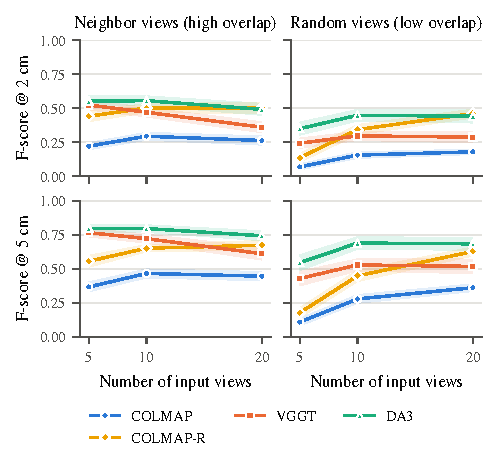
\includegraphics[width=\linewidth]{figures/fig_fscore_views.pdf}
\caption{F-score versus number of input views. Shaded: standard error over scenes and seeds. Failed
reconstructions count as zero.}
\label{fig:fscore}
\end{figure}

\begin{figure}[t]
\centering
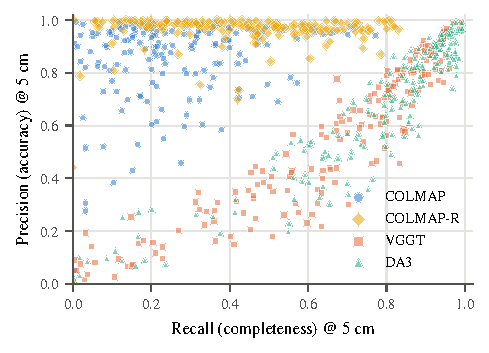
\includegraphics[width=\linewidth]{figures/fig_prec_recall.pdf}
\caption{Precision and recall at 5\,cm of every reconstruction from 5, 10 and 20 views.}
\label{fig:pr}
\end{figure}

\begin{figure*}[t]
\centering
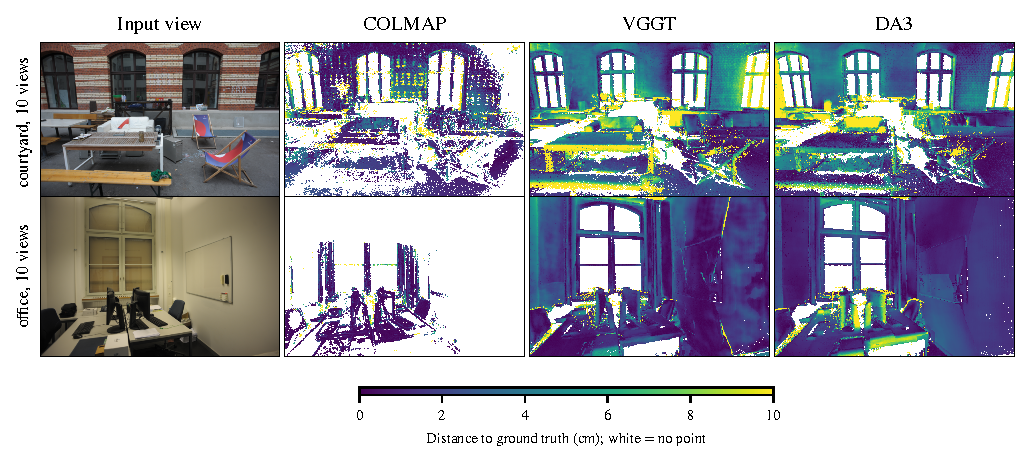
\includegraphics[width=\linewidth]{figures/fig_qualitative.pdf}
\caption{Point clouds from ten neighboring views, seen from one of the input cameras and colored by the distance
to the ground truth. White: no point. Only pixels with ground truth are evaluated, so regions without it, such as
the windows, are white for every method.}
\label{fig:qual}
\end{figure*}

DA3 has the highest F-score in every setting and at every threshold, followed by VGGT
(Table~\ref{tab:main}, Figure~\ref{fig:fscore}). The order is the same with all views, where COLMAP reaches an
F-score of 52\% at 5\,cm against 61\% for VGGT and 77\% for DA3.

Precision and recall show where the difference comes from (Figure~\ref{fig:pr}). COLMAP has the highest precision
with ten or more input views (81--86\% at 5\,cm), and with neighboring views the median distance from its points
to the ground truth is 9--14\,mm, against 20--31\,mm for DA3 and 21--44\,mm for VGGT. Its recall, however, stays at
26--40\% even with neighboring views, while DA3 recovers 84--90\% of the visible surface. Stereo fusion keeps a
point only if several depth maps agree on it, so COLMAP leaves holes wherever matching is ambiguous: on weakly
textured surfaces such as the walls in \emph{office}, at grazing angles and in regions seen by few images
(Figure~\ref{fig:qual}). The feed-forward models predict depth for every pixel, including these regions.

\paragraph{More views.}
With neighboring views, COLMAP improves from 5 to 10 views and then stays at the same level; with random views it
keeps improving, because more images get registered. The feed-forward models
become worse from 10 to 20 neighboring views (VGGT from 72\% to 61\% at 5\,cm, DA3 from 80\% to 74\%). Larger
subsets also cover more of the scene: the median angle between the viewing directions of two images grows from
$20^\circ$ for 5 views to $57^\circ$ for 20 views, and the far end of the depth range (95th percentile) from 9 to
14\,m. To separate the effect of more input views from that of a larger scene, we use the fact that our neighbor
subsets are nested: the 5 views of a subset are also contained in the 10- and 20-view subsets with the same
seed. We cut the predictions for these 5 views out of the larger reconstructions and evaluate them exactly like a
5-view reconstruction (Table~\ref{tab:nested}). On the same five images, the geometry of both feed-forward models
stays the same with more input views, so their drop in Table~\ref{tab:main} comes from the additional, harder
parts of the scene. Their cameras do not profit from the additional views either, and VGGT's become clearly
worse with 20 views. COLMAP behaves the opposite way: with 10 or 20 input views, the relative poses of the same
five images are much more accurate, because bundle adjustment uses all views and more images get registered.

\begin{table}[t]
\centering
\begin{tabular}{lcccccc}
\toprule
 & \multicolumn{3}{c}{AUC@5} & \multicolumn{3}{c}{F@5} \\
\cmidrule(lr){2-4}\cmidrule(lr){5-7}
Input views & 5 & 10 & 20 & 5 & 10 & 20 \\
\midrule
COLMAP & 62.6 & 78.4 & 78.6 & -- & -- & -- \\
VGGT & 62.3 & 62.3 & 48.6 & 74.0 & 74.7 & 72.2 \\
DA3 & 71.4 & 65.9 & 66.1 & 78.5 & 81.1 & 80.5 \\
\bottomrule
\end{tabular}

\caption{The same five neighboring views, reconstructed alone or as part of 10 or 20 input views (24 subsets).
COLMAP's fused point cloud cannot be split by view, so only its cameras are evaluated.}
\label{tab:nested}
\end{table}

\subsection{Cameras}

Relative pose accuracy depends on the setting more than geometry does. With five neighboring views, DA3 has the
best AUC@5; from ten neighboring views on and with all views, COLMAP has (Table~\ref{tab:main}). With random views,
DA3 is best by far, because COLMAP's unregistered images count as failures. Restricted to the image pairs COLMAP
registers, its AUC@5 is the highest in every setting (62--75\% against 45--68\% for DA3), although this compares
different, and for COLMAP likely easier, sets of pairs. At the coarser AUC@30, DA3 is the best or within 0.2 points
of COLMAP everywhere: its cameras are rarely far off, but less precise than those of a well-registered COLMAP
reconstruction. VGGT loses accuracy steadily with more views, from 64\% AUC@5 with 5 neighboring views to 41\% with
20 and 44\% with all views.

\subsection{Scene type}

\begin{table*}[t]
\centering
\begin{tabular}{lcrcc ccc ccc}
\toprule
 & & & \multicolumn{2}{c}{COLMAP reg.} & \multicolumn{3}{c}{F@5, neighbor 5--20} & \multicolumn{3}{c}{F@5, all views} \\
\cmidrule(lr){4-5}\cmidrule(lr){6-8}\cmidrule(lr){9-11}
Scene & Type & SIFT kp. & nb. & rand. & COLMAP & VGGT & DA3 & COLMAP & VGGT & DA3 \\
\midrule
courtyard & out & 10.2k & 97 & 62 & 27.7 & 50.9 & \textbf{58.9} & \textbf{58.2} & 37.0 & 54.3 \\
delivery\_area & out & 9.3k & 100 & 51 & 41.9 & 61.6 & \textbf{75.3} & 16.8 & 41.6 & \textbf{57.9} \\
electro & out & 10.6k & 99 & 68 & 43.0 & \textbf{75.6} & 72.3 & 60.1 & 68.3 & \textbf{72.6} \\
facade & out & 10.0k & 99 & 58 & 36.9 & 47.9 & \textbf{57.6} & \textbf{65.8} & 30.9 & 58.4 \\
playground & out & 10.3k & 70 & 33 & 35.0 & 59.9 & \textbf{68.0} & 59.5 & 43.6 & \textbf{69.8} \\
kicker & in & 10.2k & 98 & 75 & 37.0 & 85.6 & \textbf{90.0} & 39.1 & 87.3 & \textbf{91.4} \\
office & in & 5.1k & 98 & 66 & 28.7 & 93.1 & \textbf{96.2} & 35.1 & 90.3 & \textbf{97.3} \\
pipes & in & 9.9k & 85 & 67 & 45.9 & 85.7 & \textbf{91.6} & 39.6 & 84.2 & \textbf{87.4} \\
relief & in & 11.2k & 97 & 63 & 58.0 & 79.0 & \textbf{85.8} & 56.7 & 72.2 & \textbf{82.8} \\
relief\_2 & in & 10.9k & 98 & 72 & 54.6 & 64.4 & \textbf{74.5} & 60.8 & 56.8 & \textbf{86.5} \\
terrains & in & 10.8k & 100 & 56 & 67.4 & 80.6 & \textbf{95.6} & 78.8 & 62.0 & \textbf{83.0} \\
\bottomrule
\end{tabular}

\caption{Per-scene results. SIFT kp.: mean number of SIFT keypoints per image. COLMAP reg.: share of registered
images (\%) for neighbor and random subsets. F@5: F-score at 5\,cm (\%), averaged over neighbor subsets of 5, 10
and 20 views, and with all views.}
\label{tab:scene}
\end{table*}

All methods are better on the six indoor scenes than on the five outdoor ones (Table~\ref{tab:scene}). With
neighboring views, DA3 reaches an average F-score at 5\,cm of 90\% indoors and 66\% outdoors, VGGT 82\% and 59\%,
COLMAP 48\% and 37\%. Outdoor scenes are deeper (median depth 5.7\,m against 2.7\,m indoors), so a given relative depth error becomes a
larger absolute error. The outdoor scenes are also where COLMAP gets closest: with all views it has the best
F-score on \emph{courtyard} and \emph{facade}, the two scenes with the largest depth and many images (38 and 76).

Weak texture affects the classical pipeline most. \emph{office} gives about half as many SIFT keypoints as the
other scenes (5.1k per image). COLMAP still registers almost all neighboring views there, but its recall is the
lowest of all scenes, because PatchMatch finds no reliable matches on the white walls and the whiteboard
(Figure~\ref{fig:qual}). DA3, which does not rely on matching, has its best result on this scene.

\subsection{Runtime and memory}

\begin{table}[t]
\centering
\setlength{\tabcolsep}{3.2pt}
\begin{tabular}{lcccccccc}
\toprule
 & \multicolumn{4}{c}{Runtime (s)} & \multicolumn{4}{c}{Peak memory (GB)} \\
\cmidrule(lr){2-5}\cmidrule(lr){6-9}
Method & 5 & 10 & 20 & all & 5 & 10 & 20 & all \\
\midrule
COLMAP & 118 & 272 & 666 & 1161 & 5.8 & 5.8 & 5.8 & 5.8 \\
VGGT & 6.0 & 11 & 24 & 30 & 9.8 & 11.3 & 11.8 & 14.1 \\
DA3 & 2.1 & 3.7 & 6.4 & 4.8 & 11.8 & 13.7 & 14.6 & 20.5 \\
VGGT-BA & -- & -- & -- & -- & -- & -- & -- & -- \\
DA3-BA & 18 & 76 & 123 & -- & 11.8 & 13.7 & 14.6 & -- \\
\bottomrule
\end{tabular}

\caption{End-to-end runtime per reconstruction (image reading included, model loading excluded; mean) and peak
GPU memory (maximum) on one A100. Columns: number of input views. 5--20 views: three scenes, neighbor subsets;
all: 11 scenes, 34 views on average.}
\label{tab:efficiency}
\end{table}

Table~\ref{tab:efficiency} lists runtime and GPU memory. COLMAP needs 2 to 11 minutes for 5 to 20 views and
19 minutes on average for all views, 70--91\% of it in PatchMatch stereo. DA3 needs 2 to 12 seconds, VGGT 6 to
56 seconds. Most of VGGT's time is spent reading the $6048\times4032$ JPEGs with its reference loader (one image at a
time); its forward pass itself takes 0.7 to 5.6 seconds. Measured end to end, the feed-forward models are 20 to
240 times faster than COLMAP. Memory behaves the other way round. COLMAP's peak is 5.8\,GB in every run, because it
processes images at a fixed resolution and one reference image at a time. The feed-forward models attend over the
tokens of all views at once, so their memory grows with the number of views, up to 14\,GB for VGGT and 20\,GB for
DA3 on the 76 images of \emph{facade}.

%-------------------------------------------------------------------------
\section{Exploratory: Combining Both Methods}

Since COLMAP is more precise and the feed-forward models are more complete, we tried to combine them. The cameras
predicted by VGGT or DA3 replace COLMAP's incremental SfM: SIFT matches are triangulated with these cameras and
refined by bundle adjustment, then PatchMatch stereo and fusion run as usual, and finally the holes of the fused
cloud are filled with the feed-forward depth, aligned to it. We tested this on two scenes (\emph{office},
\emph{courtyard}) with 5 and 10 neighboring views.

The combination did not beat DA3: the best variant reached an F-score at 2\,cm equal to DA3 on one case and
2--4 points lower on the other three. We found three reasons. First, PatchMatch with the predicted cameras alone
yields few consistent points; bundle adjustment is necessary, but with few triangulated points it gives worse
cameras than full incremental SfM, so the MVS part is less precise than COLMAP itself. Second, refining the filled
depth with a guided filter made the results worse in every case. Third, and most important, the precision
advantage of the classical pipeline is small: on the surface that COLMAP reconstructs, its median error is
4--6\,mm against 7--10\,mm for DA3. This difference of about 3\,mm is below the noise of the outdoor ground truth
(7--8\,mm), while the missing surface costs far more F-score than the higher precision gains.

%-------------------------------------------------------------------------
\section{Limitations}

We evaluate on one benchmark with 11 scenes and three random subsets per setting, so per-scene differences are
noisy, although the main trends hold across scenes. COLMAP runs with default settings; tuned parameters, for example
relaxed initialization or more lenient fusion, would likely register more images and fill more of the surface.
The feed-forward models receive the original distorted images and are evaluated with their own pinhole
intrinsics, as in the DA3 benchmark; the ETH3D lenses are close to rectilinear (the difference in back-projection is
about 2\,mm), so this has little effect. The models run at about 500 pixels width and COLMAP at 1600 pixels, and we
compare each method at its standard resolution rather than at equal resolution. The ground truth is accurate to
about 2\,mm indoors and 7--8\,mm outdoors, so differences below 1\,cm outdoors cannot be resolved. VGGT's
runtime is dominated by its image loader and would be much lower with parallel decoding.

%-------------------------------------------------------------------------
\section{Conclusion}

On ETH3D, the feed-forward models are the better choice when only a few images are available: DA3 gives the most
complete and, by F-score, the best geometry in every setting, never fails, and needs seconds instead of minutes.
The classical pipeline remains the more accurate one where it works: its points are the most precise, and its
cameras are the best on the images it registers and with dense views. Its weaknesses are coverage and robustness,
not accuracy: it misses weakly textured and sparsely observed surfaces and fails when the views overlap little.
The two families also scale differently. COLMAP's cameras improve as views are added and its memory stays constant;
the feed-forward models do not improve on a fixed set of views as more views are added, and their memory grows
with the number of views.

{\small
\bibliographystyle{ieeenat_fullname}
\bibliography{refs}
}

\end{document}
